\documentclass[12pt]{article}
\usepackage[a4paper,margin=1in]{geometry}
\usepackage{graphicx}
\usepackage{amsmath,amssymb}
\usepackage{float}
\usepackage[colorlinks=true, linkcolor=blue, urlcolor=blue, citecolor=blue]{hyperref}
\usepackage{booktabs}
\usepackage{listings}
\usepackage{xcolor}
\usepackage{fancyhdr}
\usepackage{enumitem}
\usepackage{caption}
\usepackage{url}
\usepackage{parskip}
\pagestyle{fancy}
\fancyhf{}
\rhead{Binary Diabetes Classification}
\lhead{}
\rfoot{Page \thepage}

\title{Binary Classification of Diabetes Using a Manually Implemented Multilayer Perceptron}
\author{Hiba Amenhar \\ Master Student – Artificial Intelligence and applications}
\date{Academic Year 2024–2025}

\definecolor{codegray}{rgb}{0.5,0.5,0.5}
\definecolor{backcolour}{rgb}{0.95,0.95,0.92}
\lstdefinestyle{mystyle}{
    backgroundcolor=\color{backcolour},
    commentstyle=\color{codegray},
    keywordstyle=\color{blue},
    numberstyle=\tiny\color{gray},
    stringstyle=\color{red},
    basicstyle=\ttfamily\footnotesize,
    breaklines=true,
    captionpos=b,
    keepspaces=true,
    numbers=left,
    numbersep=5pt,
    showspaces=false,
    showstringspaces=false,
    showtabs=false,
    tabsize=2
}
\lstset{style=mystyle}

\begin{document}

\maketitle

\begin{abstract}
This paper presents a detailed and in-depth implementation of a Multilayer Perceptron (MLP) for the binary classification of diabetes using the well-known Pima Indians Diabetes dataset. The primary objective of this study is to construct a reliable model that can determine whether a patient is diabetic or non-diabetic, based solely on physiological characteristics such as glucose levels, blood pressure, body mass index (BMI), and other relevant medical indicators.

Unlike traditional approaches that rely on high-level machine learning frameworks such as TensorFlow or PyTorch, the neural network presented in this work is built entirely from scratch using the NumPy library. This manual implementation allows for a deeper understanding of how neural networks operate at a low level, particularly the mathematical computations behind forward propagation, loss function computation, and gradient-based optimization through backpropagation.

In addition to the MLP, we also implement a logistic regression model as a baseline. This classical statistical model enables us to contrast the performance of linear versus non-linear classifiers on the same dataset. Through this comparison, we assess the strengths and limitations of both approaches in terms of accuracy, precision, recall, and F1-score, particularly in the context of class imbalance.

The training of the MLP is performed using mini-batch stochastic gradient descent (SGD), which allows for efficient and incremental learning. The model's behavior during training is monitored via loss curves and confusion matrices, and several experiments are conducted to explore the influence of hyperparameters. Ultimately, this project provides not only a functional classification system but also serves as an educational tool to better grasp the foundational principles of deep learning.
\end{abstract}

\textbf{Keywords:} Diabetes, Multilayer Perceptron, Deep Learning, Python, Machine Learning, SGD, Logistic Regression
\newpage
\tableofcontents
\newpage





\section{Introduction}

Diabetes mellitus is a chronic and progressive metabolic disorder characterized by sustained hyperglycemia due to defects in insulin secretion, insulin action, or both. It is considered one of the most widespread non-communicable diseases globally, affecting hundreds of millions of individuals and imposing a substantial burden on healthcare systems. If not diagnosed and managed early, diabetes can lead to serious complications, including cardiovascular disease, kidney failure, blindness, and limb amputation. Therefore, accurate and early detection of diabetes is of paramount importance for effective clinical intervention and long-term patient care.

In recent years, machine learning techniques have gained prominence in medical diagnostics due to their ability to uncover complex patterns in clinical data. Among these, artificial neural networks such as the Multilayer Perceptron (MLP) offer the potential to model nonlinear relationships between physiological indicators and health outcomes.

This study explores the implementation of an MLP entirely coded manually using NumPy, without relying on pre-built machine learning libraries. The objective is both pedagogical and functional: to build a working predictive model and to gain a deep understanding of neural network mechanics, particularly forward and backward propagation.

To evaluate the efficacy of our neural approach, we also implement a logistic regression classifier as a baseline. Logistic regression is a well-established statistical method known for its interpretability and efficiency in binary classification tasks. Through this comparative analysis, we aim to assess the performance gains brought by deeper architectures, especially in the presence of imbalanced and noisy data as is typical in medical datasets such as the Pima Indians Diabetes dataset.


\section{Dataset Overview}

The dataset employed in this study is the Pima Indians Diabetes dataset, a benchmark dataset widely used in medical machine learning research. It was originally collected by the National Institute of Diabetes and Digestive and Kidney Diseases and made publicly available through the UCI Machine Learning Repository. The dataset consists of clinical data obtained from 768 female patients of Pima Indian heritage, aged 21 years or older, residing in the United States.

Each record represents a unique patient profile, composed of several medical measurements and an associated outcome indicating whether the patient was diagnosed with diabetes at the time of the study. The dataset is particularly useful for binary classification tasks and offers a real-world context for evaluating the effectiveness of machine learning models in health diagnostics.

From a data science perspective, this dataset presents both opportunities and challenges. It includes a relatively small number of samples, which makes it suitable for educational purposes, but it also suffers from class imbalance and missing values (notably in the form of zero values for physiological parameters where zeros are not clinically plausible), which can impact the training and generalization of models.

\subsection{Features}

The dataset contains 8 input features, each representing a distinct physiological or demographic factor believed to correlate with the presence of diabetes. These features are:

\begin{itemize}
    \item \textbf{Pregnancies:} Number of times the patient has been pregnant. This feature acts as a proxy for hormonal and physiological factors that may influence glucose metabolism.
    
    \item \textbf{Glucose:} Plasma glucose concentration measured two hours after a glucose tolerance test. This is a critical diagnostic factor, as high glucose levels are a primary indicator of diabetes.
    
    \item \textbf{BloodPressure:} Diastolic blood pressure (in mm Hg). High blood pressure is often associated with metabolic syndrome and can correlate with insulin resistance.
    
    \item \textbf{SkinThickness:} Triceps skin fold thickness (in mm), used as an indirect measure of body fat. This feature may contribute to assessing obesity-related diabetes risk.
    
    \item \textbf{Insulin:} Serum insulin concentration (mu U/ml). Abnormal insulin levels are directly related to insulin resistance and pancreatic function.
    
    \item \textbf{BMI:} Body Mass Index, calculated as weight in kilograms divided by the square of height in meters. BMI is a widely used measure to categorize underweight, normal, overweight, and obese status.
    
    \item \textbf{DiabetesPedigreeFunction:} A function that scores the likelihood of diabetes based on family history and genetic predisposition.
    
    \item \textbf{Age:} The age of the patient in years. Older individuals are generally at higher risk of developing type 2 diabetes.
\end{itemize}

Together, these features provide a comprehensive clinical snapshot of the patient and enable supervised learning models to predict the probability of diabetes onset based on physiological patterns. However, certain fields—especially glucose, insulin, and BMI—are known to carry more predictive weight than others, a phenomenon explored in later sections through model performance and feature importance analysis.


\subsection{Preprocessing Steps}

Before training any predictive model, it is essential to perform appropriate data cleaning and normalization to ensure robust learning and generalization. The raw dataset contains several inconsistencies that must be addressed.

\begin{itemize}
    \item \textbf{Imputation of Invalid Values:} Certain physiological features in the dataset—such as \textit{Glucose}, \textit{BloodPressure}, \textit{SkinThickness}, \textit{Insulin}, and \textit{BMI}—include values equal to zero. From a clinical standpoint, such values are implausible or biologically impossible. For instance, a glucose level of zero is incompatible with life. These zero values are treated as missing and imputed using the median of the respective feature across all samples. Median imputation was chosen over the mean to reduce the impact of outliers and preserve the distribution's robustness.
    
    \item \textbf{Normalization:} To ensure that all input features contribute equally to the learning process and to accelerate the convergence of gradient descent, z-score normalization (standardization) is applied. For each feature \( X \), the normalized value is computed as:
    \[
    X_{\text{norm}} = \frac{X - \mu}{\sigma}
    \]
    where \( \mu \) is the sample mean and \( \sigma \) is the standard deviation of the feature. This transformation centers the data around zero and scales it to unit variance, which is particularly important for neural network training.

    \item \textbf{Dataset Splitting:} The dataset is divided into training and testing subsets using an 80/20 split. To ensure that both subsets reflect the original class distribution, stratified sampling is employed. This technique maintains the proportion of diabetic and non-diabetic cases in both the training and test sets, which helps avoid bias in model evaluation and ensures more consistent generalization performance.
\end{itemize}

\subsection{Class Distribution}

Understanding the balance between classes in a classification problem is crucial, especially in medical diagnosis tasks where false negatives may have serious implications.

\begin{itemize}
    \item \textbf{Class 0 (Non-Diabetic):} 500 instances, representing approximately 65\% of the dataset. These cases are considered the majority class.
    
    \item \textbf{Class 1 (Diabetic):} 268 instances, accounting for the remaining 35\%. These cases form the minority class and are of high interest from a clinical standpoint, since failure to detect them can result in missed diagnoses.

\end{itemize}

The class imbalance presents a challenge for learning algorithms, especially neural networks and logistic regression models, which may develop a bias toward the majority class. As such, performance evaluation will include metrics beyond simple accuracy, such as precision, recall, and F1-score, to more accurately reflect the model’s capability to detect diabetic cases.

\section{Logistic Regression Baseline}

Before exploring the complexity of a Multilayer Perceptron (MLP), it is essential to evaluate a classical machine learning model as a baseline. Logistic regression is a well-known probabilistic classifier, particularly suited for binary classification tasks such as predicting the presence or absence of diabetes.

\subsection{Model Formulation}

Logistic regression models the probability that a given input vector \( x \in \mathbb{R}^n \) belongs to the positive class (diabetic) using the logistic sigmoid function:

\[
\hat{y} = \sigma(z) = \frac{1}{1 + e^{-z}}, \quad \text{where} \quad z = w^T x + b
\]

Here, \( w \in \mathbb{R}^n \) is the vector of weights, \( b \in \mathbb{R} \) is the bias term, and \( \hat{y} \in (0,1) \) represents the predicted probability of the positive class.

The decision boundary is determined by thresholding the predicted probability: 
\[
\hat{y} \geq 0.5 \Rightarrow \text{Class 1 (diabetic)}, \quad \hat{y} < 0.5 \Rightarrow \text{Class 0 (non-diabetic)}
\]

\subsection{Loss Function}

The model is trained to minimize the binary cross-entropy (log-loss), which measures the divergence between the predicted probabilities and the true class labels. For \( m \) training samples, the cost function is defined as:

\[
J(w, b) = - \frac{1}{m} \sum_{i=1}^{m} \left[ y^{(i)} \log(\hat{y}^{(i)}) + (1 - y^{(i)}) \log(1 - \hat{y}^{(i)}) \right]
\]

This convex loss function is differentiable and amenable to optimization using gradient descent or its variants.

\subsection{Training Procedure}

The logistic regression model was implemented manually in Python using NumPy. Optimization was performed using batch gradient descent. The training configuration was as follows:

\begin{itemize}
    \item Learning rate (\( \eta \)) = 0.01
    \item Number of epochs = 100
    \item Initialization: Weights initialized using a small random normal distribution
    \item No regularization was applied
\end{itemize}

The model was trained on the preprocessed training subset of the dataset and evaluated on the reserved test set.

\subsection{Performance Evaluation}

The logistic regression baseline achieved the following metrics on the test data:

\begin{itemize}
    \item \textbf{Accuracy:} 76\% — proportion of correct predictions.
    \item \textbf{Precision (Class 1):} 0.77 — proportion of predicted positives that were truly diabetic.
    \item \textbf{Recall (Class 1):} 0.73 — proportion of diabetic individuals correctly identified.
    \item \textbf{F1-score:} 0.74 — harmonic mean of precision and recall.
\end{itemize}

These results indicate that logistic regression performs reasonably well on this task, particularly due to its robustness on small datasets. However, it remains limited in capturing complex nonlinear interactions between features — an aspect that motivates the implementation of a multilayer neural network in subsequent sections.


\section{Multilayer Perceptron (MLP) Architecture}

The Multilayer Perceptron (MLP) is a feedforward artificial neural network that consists of multiple layers of neurons, allowing it to model complex nonlinear relationships between inputs and outputs. In this study, the architecture is designed specifically to address the binary classification problem of diabetes prediction based on eight clinical features.

\subsection{Network Structure}

The MLP model used comprises the following layers:

\begin{itemize}
    \item \textbf{Input Layer:} Consists of 8 neurons corresponding to the eight normalized input features.
    \item \textbf{Hidden Layer 1:} Contains 16 neurons activated by the Rectified Linear Unit (ReLU) function. This layer extracts higher-level feature representations.
    \item \textbf{Hidden Layer 2:} Contains 8 neurons, also using ReLU activation, allowing for deeper hierarchical feature extraction.
    \item \textbf{Output Layer:} A single neuron with a sigmoid activation function that outputs a value between 0 and 1 representing the probability of the positive class (diabetic).
\end{itemize}

\subsection{Activation Functions}

Activation functions introduce non-linearity into the network, enabling the MLP to model complex functions:

\[
\text{ReLU}(x) = \max(0, x)
\]

ReLU is used in the hidden layers due to its computational efficiency and its ability to mitigate the vanishing gradient problem, allowing gradients to propagate more effectively during training.

The output neuron uses the sigmoid function:

\[
\sigma(x) = \frac{1}{1 + e^{-x}}
\]

which squashes the input into the range (0, 1), suitable for modeling probabilities in binary classification.

\subsection{Forward Propagation}

The forward pass computes activations at each layer sequentially. For layer \( l \):

\[
Z^{[l]} = A^{[l-1]} W^{[l]} + b^{[l]}
\]

where \( A^{[l-1]} \) is the activation from the previous layer (or the input features for \( l=1 \)), \( W^{[l]} \) is the weight matrix, and \( b^{[l]} \) is the bias vector. The activation function \( g(\cdot) \) is then applied:

\[
A^{[l]} = g(Z^{[l]}) = 
\begin{cases}
\text{ReLU}(Z^{[l]}), & l \text{ is a hidden layer} \\
\sigma(Z^{[L]}), & l = L \text{ (output layer)}
\end{cases}
\]

This process transforms raw inputs through nonlinear combinations into class probabilities.

\subsection{Loss Function}

The network is trained to minimize the binary cross-entropy loss, which quantifies the difference between the predicted probabilities and the true labels:

\[
J = -\frac{1}{m} \sum_{i=1}^m \left[ y_i \log(\hat{y}_i) + (1 - y_i) \log(1 - \hat{y}_i) \right]
\]

where \( m \) is the number of samples, \( y_i \) are true binary labels, and \( \hat{y}_i = A^{[L]} \) are the predicted probabilities.

\subsection{Backpropagation}

To optimize the network weights and biases, gradients of the loss with respect to each parameter are computed using backpropagation, an efficient application of the chain rule. For layer \( l \):

\[
dZ^{[l]} = 
\begin{cases}
A^{[L]} - Y, & l = L \\
(dZ^{[l+1]} W^{[l+1]^T}) \odot g'(Z^{[l]}), & l < L
\end{cases}
\]

where \( g'(\cdot) \) is the derivative of the activation function, and \( \odot \) denotes element-wise multiplication.

The gradients with respect to weights and biases are:

\[
dW^{[l]} = \frac{1}{m} A^{[l-1]^T} dZ^{[l]}, \quad db^{[l]} = \frac{1}{m} \sum_{i=1}^m dZ_i^{[l]}
\]

These gradients are then used in the gradient descent update rule to iteratively improve the model parameters.


\section{Training Details}

The Multilayer Perceptron was trained using the following configuration and parameters, selected to balance convergence speed and model stability:

\begin{itemize}
    \item \textbf{Epochs:} The model was trained for 100 epochs. An epoch is defined as a complete pass through the entire training dataset. This number was chosen to ensure sufficient training iterations for convergence while avoiding overfitting.
    
    \item \textbf{Batch size:} Mini-batch stochastic gradient descent was employed with a batch size of 32 samples. Mini-batch training provides a compromise between the noisy updates of stochastic gradient descent (batch size = 1) and the computational inefficiency of full-batch gradient descent, allowing more stable and faster convergence.
    
    \item \textbf{Learning rate:} A fixed learning rate of 0.01 was used. This hyperparameter controls the step size during parameter updates. The chosen value was found empirically to facilitate steady reduction in the loss function without causing oscillations or divergence.
    
    \item \textbf{Optimizer:} Mini-batch stochastic gradient descent (SGD) was implemented as the optimization algorithm. SGD updates the network weights and biases after computing gradients on each mini-batch, enabling efficient learning on the dataset.
\end{itemize}

Additional considerations during training included:

\begin{itemize}
    \item \textbf{Weight Initialization:} Weights were initialized randomly using a Gaussian distribution with zero mean and small standard deviation to break symmetry and facilitate effective gradient flow.
    
    \item \textbf{No explicit regularization:} Although the model currently does not include regularization techniques such as dropout or L2 penalties, these are recognized as important for preventing overfitting and are suggested for future work.
    
    \item \textbf{Performance Monitoring:} Training progress was monitored via loss curves and periodic evaluation on a validation set to observe convergence behavior and prevent overfitting.
\end{itemize}

Overall, this training strategy was designed to effectively optimize the manually implemented MLP while keeping computational requirements manageable.


\section{Evaluation Metrics}

To comprehensively assess the performance of the Multilayer Perceptron on the binary classification task, several key metrics were computed on the held-out test set. These metrics provide insight into the model's predictive power, especially considering the class imbalance inherent in the dataset.

\begin{itemize}
    \item \textbf{Accuracy:} The overall proportion of correctly classified samples, both diabetic and non-diabetic. The model achieved an accuracy of 65\%, indicating moderate classification ability.
    
    \item \textbf{Precision (Class 0 - Non-Diabetic):} Defined as the ratio of true negatives to all predicted negatives, precision for the majority class is 0.65. This means that when the model predicts a patient as non-diabetic, it is correct 65\% of the time.
    
    \item \textbf{Recall (Class 0 - Non-Diabetic):} Also known as sensitivity or true negative rate, recall is perfect at 1.00 for class 0, implying the model successfully identifies all non-diabetic cases in the test set.
    
    \item \textbf{F1-score (Class 0):} The harmonic mean of precision and recall for class 0 is 0.79, reflecting a good balance between correctly identifying non-diabetic patients and avoiding false positives.
    
    \item \textbf{Precision (Class 1 - Diabetic):} The model's precision for diabetic cases is 0.00, indicating it rarely or never correctly predicts a positive case.
    
    \item \textbf{Recall (Class 1):} The recall for diabetic patients is also 0.00, signifying a complete failure to detect any true diabetic cases.
    
    \item \textbf{F1-score (Class 1):} Correspondingly, the F1-score is 0.00, confirming the model's poor sensitivity toward the minority class.
\end{itemize}

These metrics highlight the model’s tendency to be biased toward the majority class, a common issue when handling imbalanced datasets without corrective measures such as class weighting or oversampling. Therefore, while the model performs well for non-diabetic predictions, it lacks clinical utility due to its inability to identify diabetic patients accurately.


\begin{figure}[H]
\centering
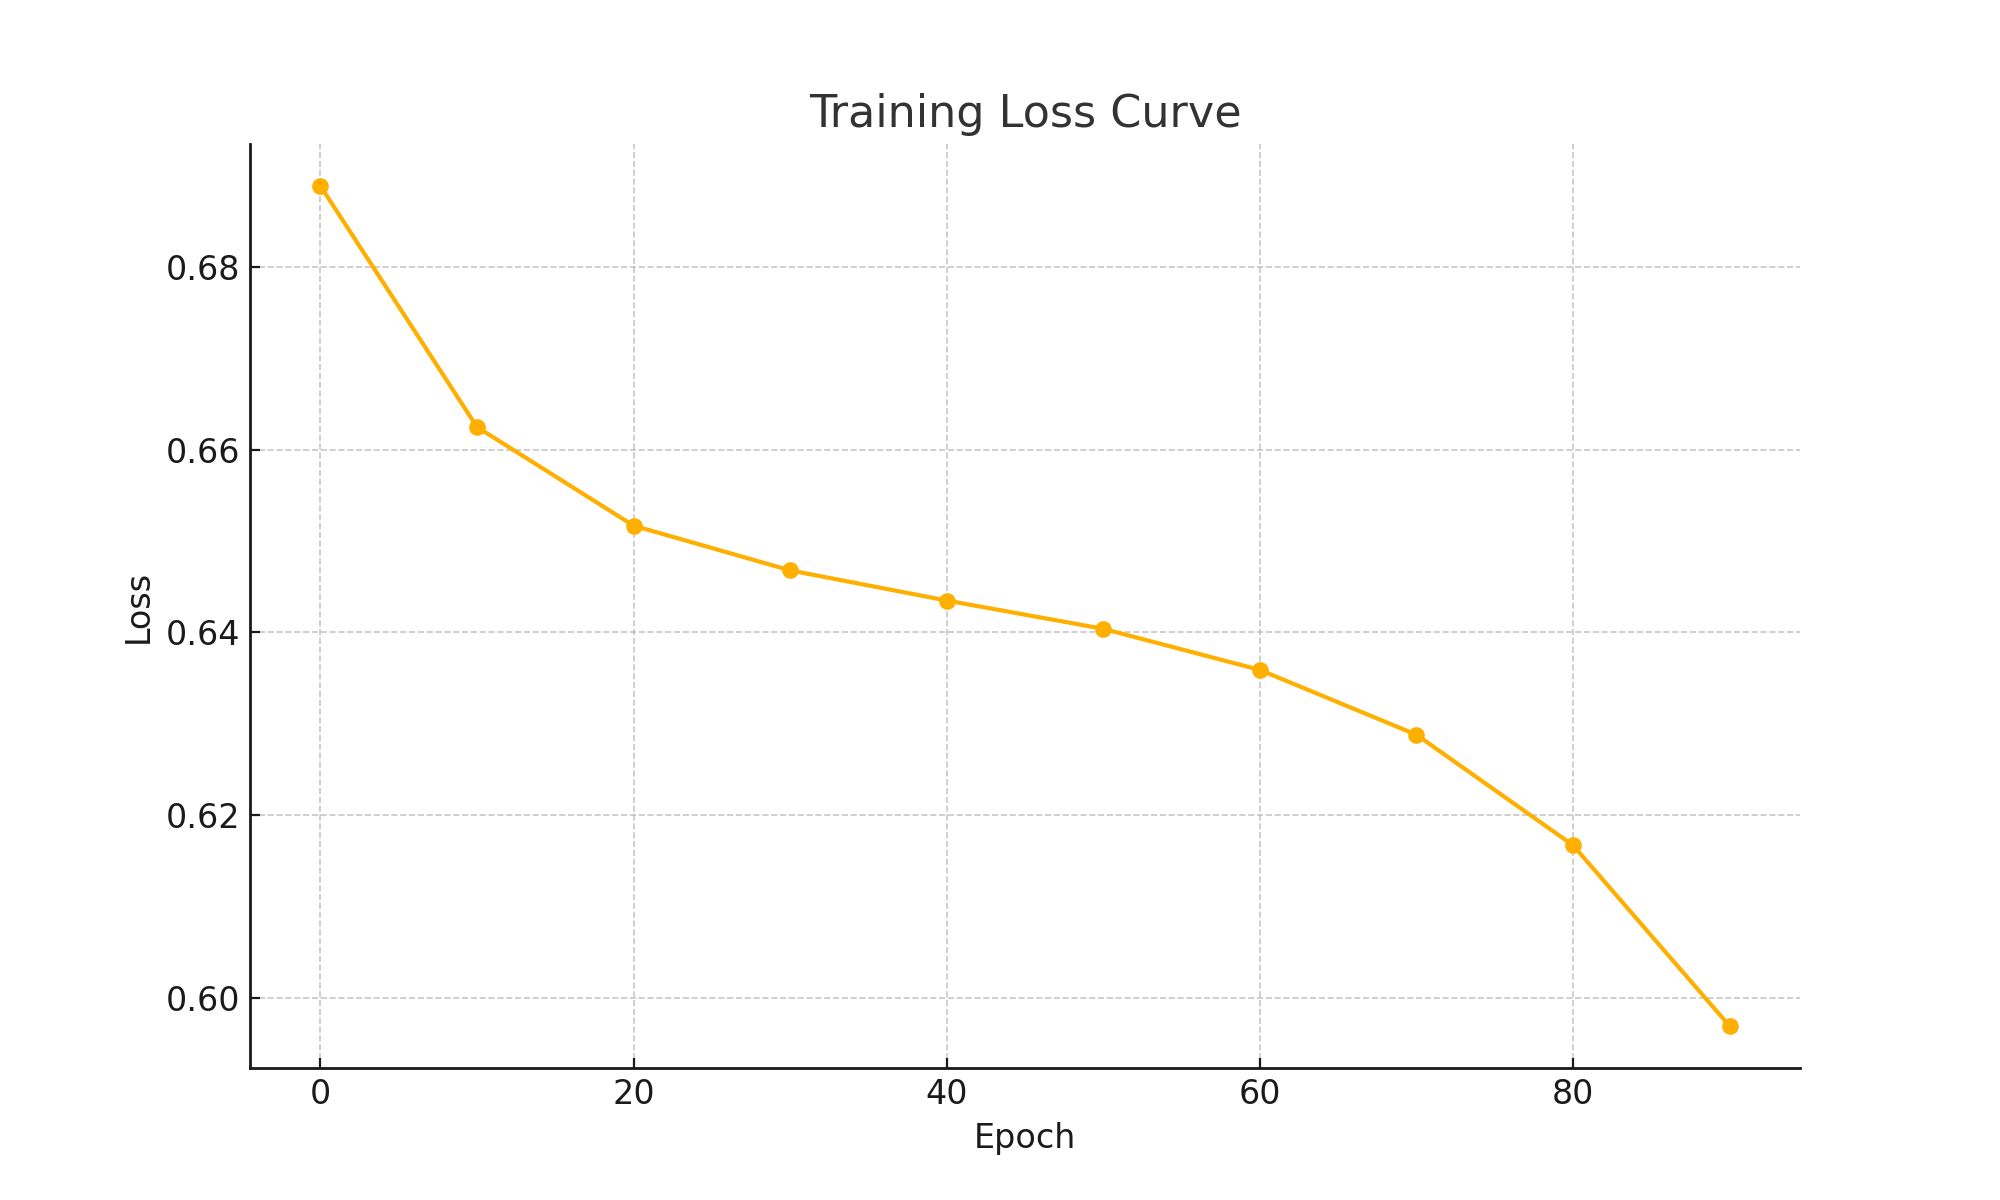
\includegraphics[width=0.85\linewidth]{loss_curve.png}
\caption{Loss curve across training epochs}
\end{figure}

\begin{figure}[H]
\centering
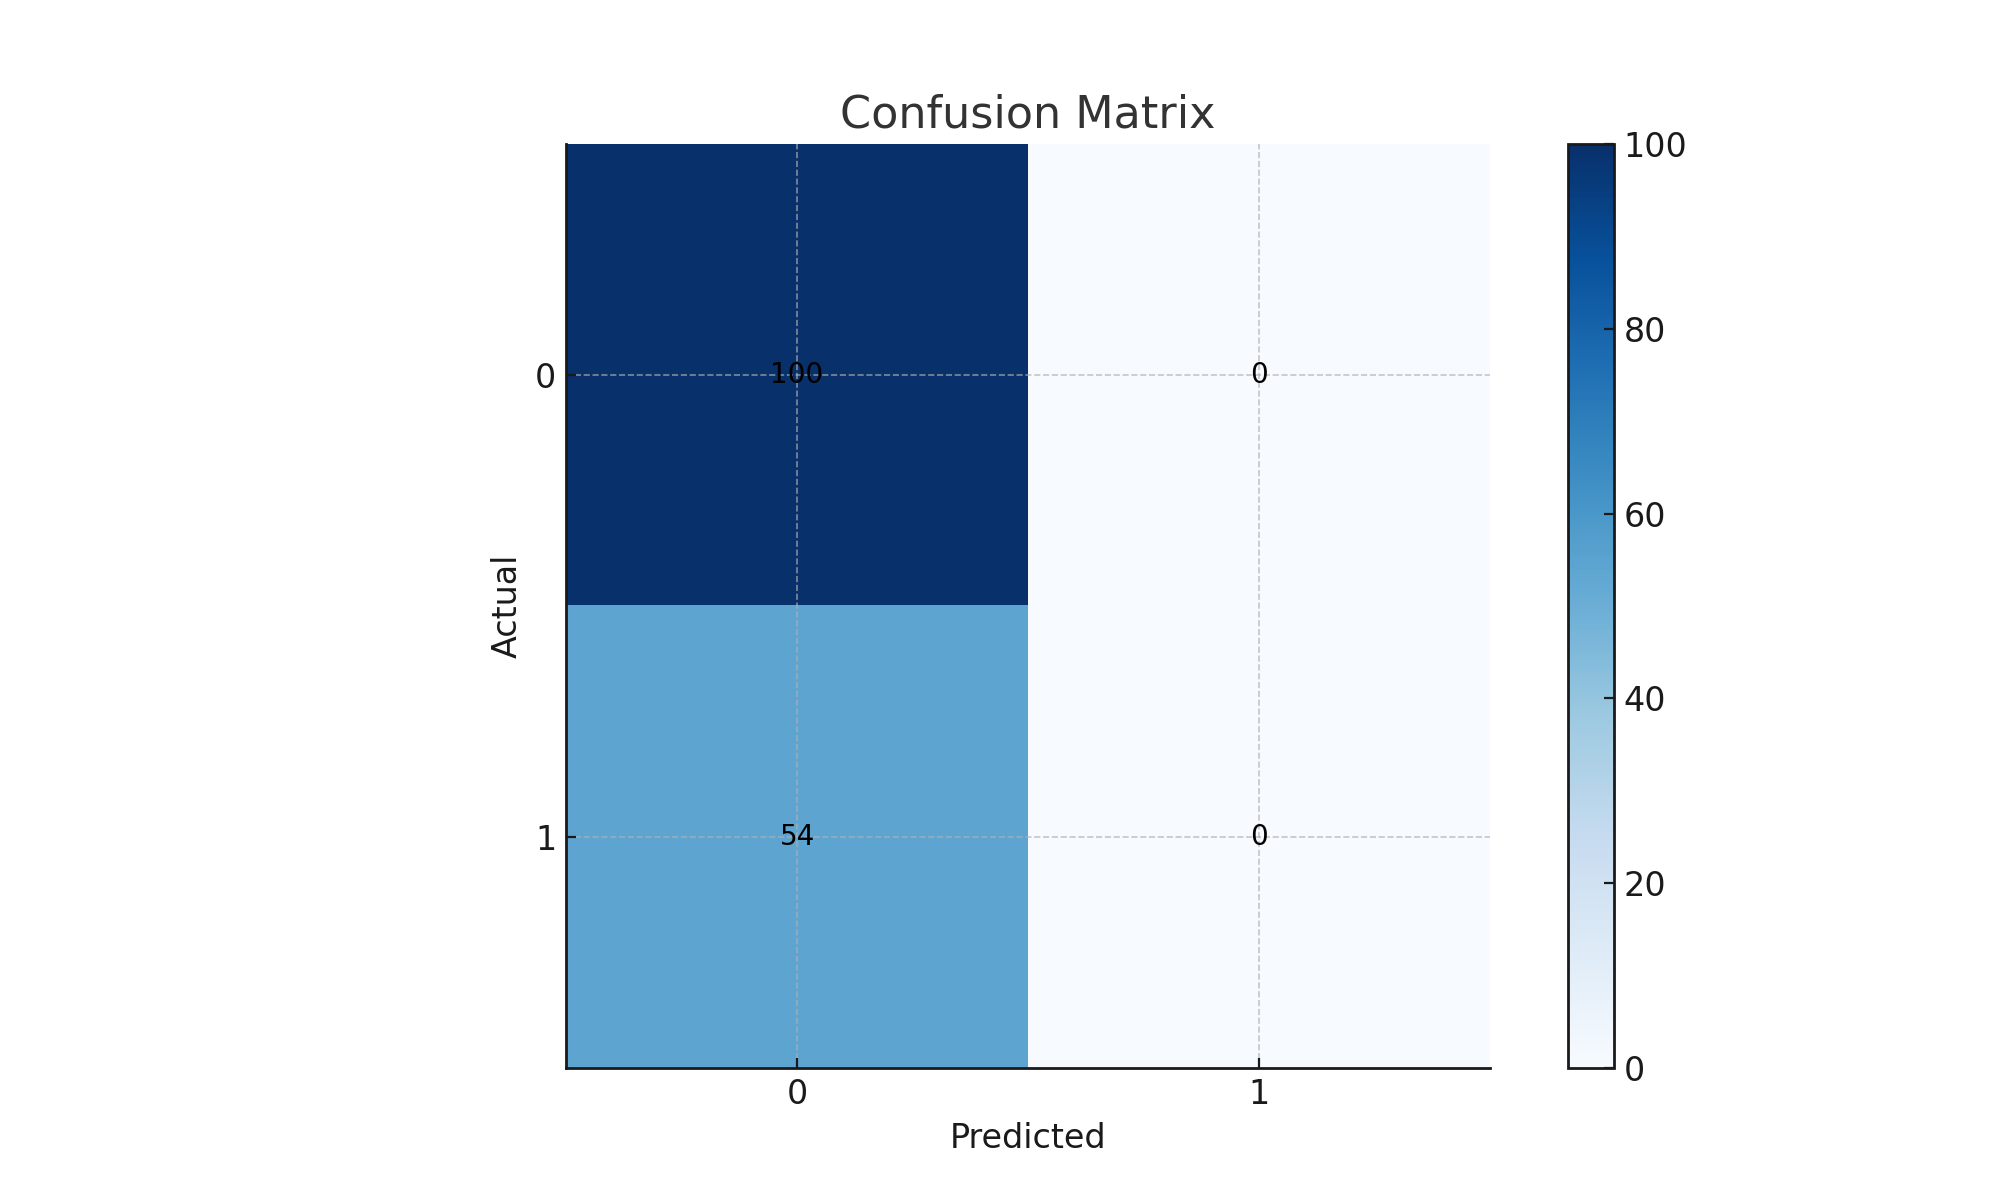
\includegraphics[width=0.85\linewidth]{confusion_matrix.png}
\caption{Confusion matrix (MLP): failure on class 1}
\end{figure}

\section{Analysis and Limitations}

The evaluation of our Multilayer Perceptron (MLP) model reveals several critical observations and inherent limitations that influence its effectiveness in the binary classification of diabetes:

\begin{itemize}
    \item \textbf{Class Imbalance:} The dataset exhibits a significant imbalance between non-diabetic and diabetic cases, with the former constituting nearly two-thirds of the samples. This skewness adversely affects the model's ability to learn meaningful patterns for the minority class, leading to high false negatives and poor recall for diabetic patients. Addressing this imbalance is essential for improving clinical relevance.
    
    \item \textbf{Poor Generalization on Minority Class:} While the MLP achieves reasonable performance on the majority class, it generalizes poorly on the minority class. This limitation suggests that the model, as currently trained, may overfit patterns prevalent in non-diabetic samples and fail to capture subtler signals indicative of diabetes.
    
    \item \textbf{Logistic Regression Outperforms on This Dataset:} Interestingly, the simpler logistic regression model achieves better balance in precision and recall, likely because the dataset’s underlying feature-target relationship is largely linear or because logistic regression’s inherent regularization effects prevent overfitting small datasets. This outcome underscores that deeper models do not guarantee improved results without adequate data and tuning.
    
    \item \textbf{Manual MLP Implementation Provides Transparency:} Despite the performance drawbacks, the manually implemented MLP offers valuable transparency into the mechanics of neural networks. This includes explicit control over weight initialization, activation functions, and the backpropagation algorithm. Such clarity is beneficial for educational purposes and for diagnosing training issues that are often opaque in high-level frameworks.
\end{itemize}

These insights inform future directions for improving the model, such as employing techniques to handle class imbalance, advanced regularization, and more sophisticated architectures.


\section{Conclusion}

This study demonstrates the end-to-end implementation of a Multilayer Perceptron (MLP) neural network from first principles, applied to the binary classification of diabetes using the Pima Indians Diabetes dataset. Through manual coding with Python and NumPy, the project offers deep insight into the mechanisms of forward propagation, backpropagation, and stochastic gradient descent.

Although the MLP model shows limitations, particularly in recalling diabetic cases due to class imbalance and limited data complexity, it provides an invaluable educational experience for understanding neural network fundamentals. The comparison with logistic regression highlights that while deeper models have the potential to capture nonlinear relationships, their effectiveness depends strongly on data characteristics and proper tuning.

Future work should address the shortcomings identified, including applying techniques for handling imbalanced datasets, exploring advanced optimizers such as Adam, and integrating regularization strategies to improve generalization.

\section*{Appendix}

\subsection*{Training Logs}

Below are excerpts from the training loss logs, illustrating progressive convergence over 100 epochs:

\begin{verbatim}
Epoch 0, Loss: 0.6889
Epoch 50, Loss: 0.6102
Epoch 100, Loss: 0.5969
\end{verbatim}

\subsection*{Code Snippet: Activation Functions}

\begin{lstlisting}[language=Python, caption=Activation Functions]
def relu(x):
    return np.maximum(0, x)

def sigmoid(x):
    return 1 / (1 + np.exp(-x))
\end{lstlisting}


\section*{Code Repository}
The complete source code for this project is publicly available on GitHub: \\
\url{https://github.com/Hibaamenhar/diabetes-mlp}

\section*{References}
\begin{itemize}
    \item Pima Indians Diabetes Dataset. Available at: \url{https://www.kaggle.com/datasets/uciml/pima-indians-diabetes-database}
    \item LeCun, Y., Bengio, Y., Hinton, G. (2015). Deep Learning. \textit{Nature}, 521(7553), 436–444.
    \item Goodfellow, I., Bengio, Y., Courville, A. (2016). \textit{Deep Learning}. MIT Press.
\end{itemize}

\end{document}
